\documentclass[11pt]{article}
\usepackage{amsmath}
\usepackage{amsfonts} 
\usepackage{listings}
\usepackage{algorithm}
\usepackage{geometry}
\usepackage{mathtools}
\usepackage[slovak,shorthands=off]{babel}
\usepackage{graphicx}
\usepackage{floatpag}
\usepackage{amsthm}
\usepackage{tcolorbox}
\usepackage[noEnd=false]{algpseudocodex}
\usepackage[utf8]{inputenc} 
\usepackage[T1]{fontenc}    
\usepackage{csquotes}
\usepackage{biblatex}
\addbibresource{TexResources/references.bib}
\geometry{margin=2cm}
\pagenumbering{gobble}
\setlength{\parskip}{0.75\baselineskip}
\setlength{\parindent}{0pt}

\begin{document}


\title{RP}
\begin{center}
    {\LARGE Report ročníkový projekt zimný semester 2024/2025}\\[1em]
    {\large Alex Diko  \\ \texttt{diko3@uniba.sk}}\\[1em]
\end{center}

\paragraph{Pojmy:}

\textit{Graf} je dvojica $G = (V,E)$, kde $V,E$ sú množiny také, že $E \subseteq V\times V$
a $V \cap E = \emptyset$. Prvky $V$ sa nazývajú \textit{vrcholy} grafu $G$ a prvky $E$ jeho \textit{hrany}.
Množinu hrán grafu $G$ označujeme ako $E(G)$. Vrchol 
$v$ je \textit{incidentný} s hranou $e$, ak $v\in e$. \textit{Stupeň vrcholu} je počet
hrán s ním incidentných. Dve hrany sú \textit{susedné}, ak existuje vrchol, ktorý je 
s obidvomi incidentný. Ak všetky vrcholy grafu
majú stupeň $k$, graf sa nazýva \textit{$k$-regulárny}. \textit{Cesta} je neprázdny graf $P = (V,E)$,
kde $V = \{x_0, x_1, \ldots, x_k\}$ a $E = \{x_0x_1, x_1x_2, \ldots, x_{k-1}x_k\}$,
pričom všetky $x_i$ sú rôzne. Túto cestu označíme $x_0x_1\ldots x_k$. Ak $P = x_0\ldots x_{k-1}$ je cesta, potom
graf $C := P + x_{k-1}x_0$ sa nazýva \textit{kružnica}. \textit{Dĺžka} kružnice je počet jej hrán. Graf
$ G'(V',E')$ je \textit{podgrafom} grafu $G$ ak $V' \subseteq V$ a $E' \subseteq E$.
\textit{Rozklad} množiny $E(G)$ je množina $R = \{R_1, \ldots, R_k\}$, kde $R_i$
sú navzájom disjunktné a zjednotenie $\cup R$ všetkých množín $R_i \in R$ sa rovná $E(G)$. \cite{diestel2024graph}

\textit{Kružnicovou dekompozíciou grafu} nazveme rozklad $E(G)$ na kružnice, ktoré nezdieľajú žiadnu
hranu. Ak každá kružnica tohto rozkladu má párnu dĺžku, nazveme tento rozklad \textit{párnym} (ďalej
\textit{ECD} z anglického \textit{Even cycle decomposition}).
Pre ECD grafu zafarbíme každú jeho kružnicu tak, aby kružnice so spoločným
vrcholom nemali rovnakú farbu. Potom zjednotenie kružníc v každej farebnej triede 
bude 2-regulárny podgraf pôvodného grafu. Ak najmenší počet farieb potrebných 
na takéto zafarbenie je $m$ potom ECD rozklad má \textit{veľkosť} $m$. \cite{MALNEGRO2024113844}

\begin{figure}[h]
    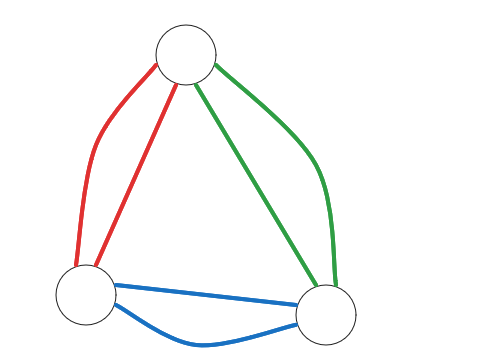
\includegraphics[scale=0.4]{TexResources/2c3ecd}
    \centering
    \caption{ECD rozklad veľkosti 3 na červenú, modrú a zelenú kružnicu}
\end{figure}
\paragraph{Práca za semester:}
Do grafovej knižnice \texttt{ba-graph} som v jazyku \texttt{c++} naimplementoval backtracking (prehľadávanie 
s návratom) algoritmus, ktorý nájde veľkosť ECD grafu (súbor \texttt{ecd.hpp}). Pseudokód algoritmu je uvedený nižšie.
\begin{algorithmic}[1]
   
    \Function{NájdiECD}{graf}
        \State inicializuj počet farebný tried na 0
        \State \Call{SkúsZačaťNovúKružnicu}{}

        \If{žiadne ECD sa nenašlo}
            \State \Return neexistuje ECD
        \Else
            \State \Return najmenšie ECD
        \EndIf
    \EndFunction
    \State
    \Function{SkúsZačaťNovúKružnicu}{}
        \If{všetky hrany sú priradené farebnej triede}
            \State porovnaj veľkosť tohto ECD s doteraz najmenším nájdeným, ak je menšie zapamätaj si priradenie hrán do farebných tried
            \State \Return
        \Else
            \State $h \gets$ zober nejakú nepriradenú hranu \label{line:vyber}
            \ForAll{$f \in$ aktuálne farebné triedy}
                \State skús priradiť $h$ do $f$ a zapamätaj si, že $h$ bude v kružnici na párnej pozícii
                \State \Call{SkúsPokračovaťVAktuálnejKružnici}{$h$}
            \EndFor

            \State skús priradiť $h$ do novej farebnej triedy a zapamätaj si, že $h$ bude v kružnici na párnej pozícii
            \If{počet farebných tried je väčší alebo rovný ako aktuálne najmenšie nájdené ECD}
            \State odmietni aktuálne riešenie
            \State \Return
            \EndIf
            \State \Call{SkúsPokračovaťVAktuálnejKružnici}{$h$}
        \EndIf

    \EndFunction
    \State
    \Function{SkúsPokračovaťVAktuálnejKružnici}{\textit{aktuálnaHrana}}
        \LComment{Over či je aktuálnaHrana správne zafarbená. V korektnej ECD 
        musia byť práve 2 susedné hrany v rovnakej farebnej triede a na pozíciach 
        inej parity ako aktuálnaHrana}
        \State $p \gets 0$ \Comment{Počet susedných hrán v rovnakej farebnej triede ale na pozíciach
        rôznej parity}
        \ForAll{$h \in$ hrany susedné s \textit{aktuálnaHrana}}
        \If{$h$ je v rovnakej farebnej triede ako \textit{aktuálnaHrana}}
            \If{$h$ je na pozícii rovnakej parity ako \textit{aktuálnaHrana}}
            \State odmietni aktuálnu kružnicu 
            \State \Return
            \Else
            \State $p \gets p+1$
            \EndIf
        \EndIf
        \EndFor
        
        \If{$p > 2$}
        \State odmietni aktuálnu kružnicu
        \State \Return
        \ElsIf{$p = 2$}
        \State \Call{SkúsZačaťNovúKružnicu}{} \Comment{Bez sporu sa nám podarilo vytvoriť kružnicu párnej dĺžky}
        \State \Return
        \Else
        \ForAll{$h \in$ hrany susedné s \textit{aktuálnaHrana} a aktuálne nepriradené do farebnej triedy}
            \State skús priradiť $h$ do rovnakej farebnej triedy ako aktuálnaHrana ale na pozíciu inej parity
            \Call{SkúsPokračovaťVAktuálnejKružnici}{$h$}
        \EndFor
        \EndIf
        
    \EndFunction
\end{algorithmic}

K algoritmu sú urobené aj testy (\texttt{testy\_ecd.cpp}). Skúšal som viacero variant algoritmu (napríklad, že 
iterujeme cez všetky možné veľkosti ECD od najmenšej po najväčšiu a pre každú veľkosť skúšame nájsť jedno zafarbenie.
Ak ho nájdeme, skončíme.), ale tento bol najrýchlejší. Pri výbere hrany na riadku \ref{line:vyber}
máme viacej možností. Skúšal som program, kde je poradie výberu hrán náhodne a spustenia
programu na rovnakých vstupoch trvali rôzne dlho. Teda to, v akom poradí sú tam vyberané 
hrany, ovplyvňuje rýchlosť. Skúšal som heuristiku, kde sa vždy vyberie hrana, ktorá má najviac
susedov priradených do nejakej farebnej triedy. Rýchlejší bol však variant, kde sa vrcholy vyberajú
na základe poradia, v ktorom sú prehľadávané do šírky BFS algoritmom od prvej hrany, ktorá sa zafarbí.
Varianty backtrackingu sa dajú pozrieť ako rôzne \texttt{git} vetvy. 

\paragraph{Práca na letný semester:} ECD by sa malo dať nájsť pomocou SAT solvera.
\printbibliography
\end{document}
